% =======================================================================================================
\section{Resultados}
\label{sec:resultados}

Os resultados são apresentados na ordem em que um praticante os obtenharia: primeiro o desempenho
do modelo, depois o efeito de cada hiperparâmetro, depois o diagnóstico dos erros e, por fim, a
comparação com alternativas. Ao longo de toda a seção, a pergunta não é apenas ``quanto acertou'',
mas ``por quê''.

\subsection{Desempenho do modelo principal}

O modelo adotado --- MLP com uma camada oculta de 16 neurônios, ativação \emph{tanh}, $\alpha =
10^{-2}$ e otimizador Adam --- tem \parametrosMLP{} parâmetros treináveis. A
\tabela{tab:modelos} resume o desempenho dos quatro modelos avaliados; a coluna de acurácia é a
média de 25 dobras de validação cruzada repetida.

\begin{table}[htbp]
	\centering
	\caption{Comparação dos modelos sob validação cruzada estratificada repetida
	(5 dobras $\times$ 5 repetições = 25 ajustes), com as mesmas dobras para todos.}
	\label{tab:modelos}
	% gerado automaticamente por mlp_iris.py - nao editar

\begin{tabular}{lrrrr}
\toprule
\textbf{modelo} & \textbf{acurácia (\%)} & \textbf{desvio (p.p.)} & \textbf{F1 macro (\%)} & \textbf{tempo (s)} \\
\midrule
MLP & 96{,}8 & 3{,}1 & 96{,}8 & 9{,}4 \\
RF & 95{,}7 & 3{,}3 & 95{,}7 & 13{,}9 \\
GB & 95{,}6 & 3{,}2 & 95{,}6 & 15{,}7 \\
LR & 97{,}5 & 2{,}9 & 97{,}5 & 0{,}200 \\
\bottomrule
\end{tabular}

\end{table}

A MLP alcança \accMLP{} de acurácia média (desvio de \sdMLP{} entre dobras) e $F_1$ macro de
$96{,}8\,\%$. No conjunto de teste, reservado até este ponto, o resultado é de \accTeste{}
(42 acertos em \nTeste{} amostras), com $F_1$ macro de \fmacroTeste{} e entropia cruzada de
\llteste{}. O intervalo de confiança de Wilson para essa acurácia vai de \icLo{} a \icHi{}.

A diferença entre a estimativa de validação cruzada ($96{,}8\,\%$) e a do teste ($93{,}3\,\%$) é de
$3{,}5$ pontos percentuais --- cerca de 1,6 amostra. Não é um sinal de problema; é a variabilidade
esperada de um teste com 45 amostras. A \figura{fig:confusao} mostra onde estão os três erros.

\begin{figure}[htbp]
	\centering
	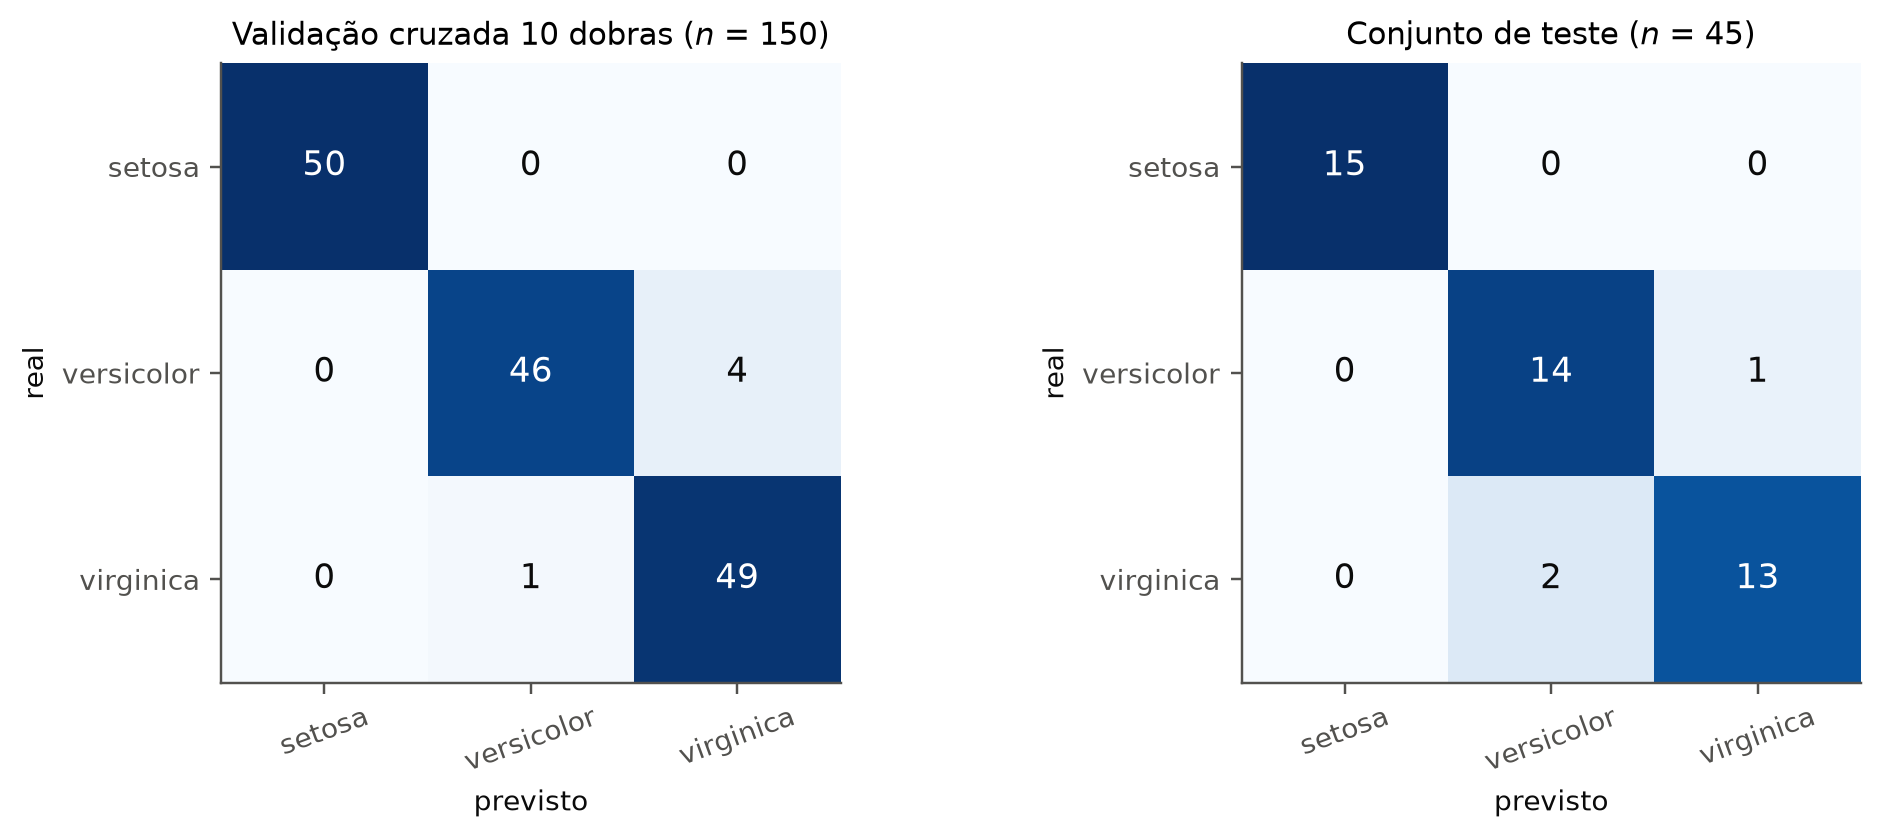
\includegraphics[width=\textwidth]{fig_confusao.png}
	\caption{Matrizes de confusão. À esquerda, previsões fora da amostra obtidas por validação
	cruzada de 10 dobras sobre as 150 amostras; à direita, o conjunto de teste de 45 amostras.}
	\label{fig:confusao}
\end{figure}

\subsection{Diagnóstico dos erros}

A matriz de confusão da validação cruzada (150 amostras) está na \tabela{tab:confusao}. Três
fatos se destacam.

\begin{table}[htbp]
	\centering
	\caption{Matriz de confusão da validação cruzada de 10 dobras (150 amostras). Linhas: classe
	real; colunas: classe prevista.}
	\label{tab:confusao}
	% gerado automaticamente por mlp_iris.py - nao editar

\begin{tabular}{lccc}
\toprule
\textbf{real $\backslash$ previsto} & \textbf{setosa} & \textbf{versicolor} & \textbf{virginica} \\
\midrule
setosa & 50 & 0 & 0 \\
versicolor & 0 & 46 & 4 \\
virginica & 0 & 1 & 49 \\
\bottomrule
\end{tabular}

\end{table}

\begin{enumerate}
	\item a \emph{setosa} é classificada perfeitamente: 50 de 50. Isso era esperado pela análise
	      exploratória, já que a classe é separável;
	\item os erros entre \emph{versicolor} e \emph{virginica} são assimétricos: quatro
	      \emph{versicolor} foram previstas como \emph{virginica} e apenas uma \emph{virginica} foi
	      prevista como \emph{versicolor}. O modelo erra mais na direção da classe de pétalas
	      maiores;
	\item não há confusão entre \emph{setosa} e qualquer outra classe, o que confirma que a rede
	      aprendeu a estrutura global antes de refinar a fronteira difícil.
\end{enumerate}

A \tabela{tab:por-classe} detalha precisão, revocação e $F_1$ por classe. A \emph{setosa} tem
$100\,\%$ nas três métricas. A \emph{versicolor} tem precisão alta ($97{,}9\,\%$) e revocação mais
baixa ($92{,}0\,\%$): quando o modelo diz \emph{versicolor}, quase sempre acerta, mas deixa passar
algumas. A \emph{virginica} mostra o padrão oposto: revocação de $98{,}0\,\%$ e precisão de
$92{,}5\,\%$.

\begin{table}[htbp]
	\centering
	\caption{Métricas por classe na validação cruzada de 10 dobras (\%).}
	\label{tab:por-classe}
	% gerado automaticamente por mlp_iris.py - nao editar

\begin{tabular}{lrrrr}
\toprule
\textbf{Classe} & \textbf{Suporte} & \textbf{Precisão} & \textbf{Revocação} & \textbf{F1} \\
\midrule
setosa & 50 & 100{,}0 & 100{,}0 & 100{,}0 \\
versicolor & 50 & 97{,}9 & 92{,}0 & 94{,}8 \\
virginica & 50 & 92{,}5 & 98{,}0 & 95{,}1 \\
\bottomrule
\end{tabular}

\end{table}

\begin{figure}[htbp]
	\centering
	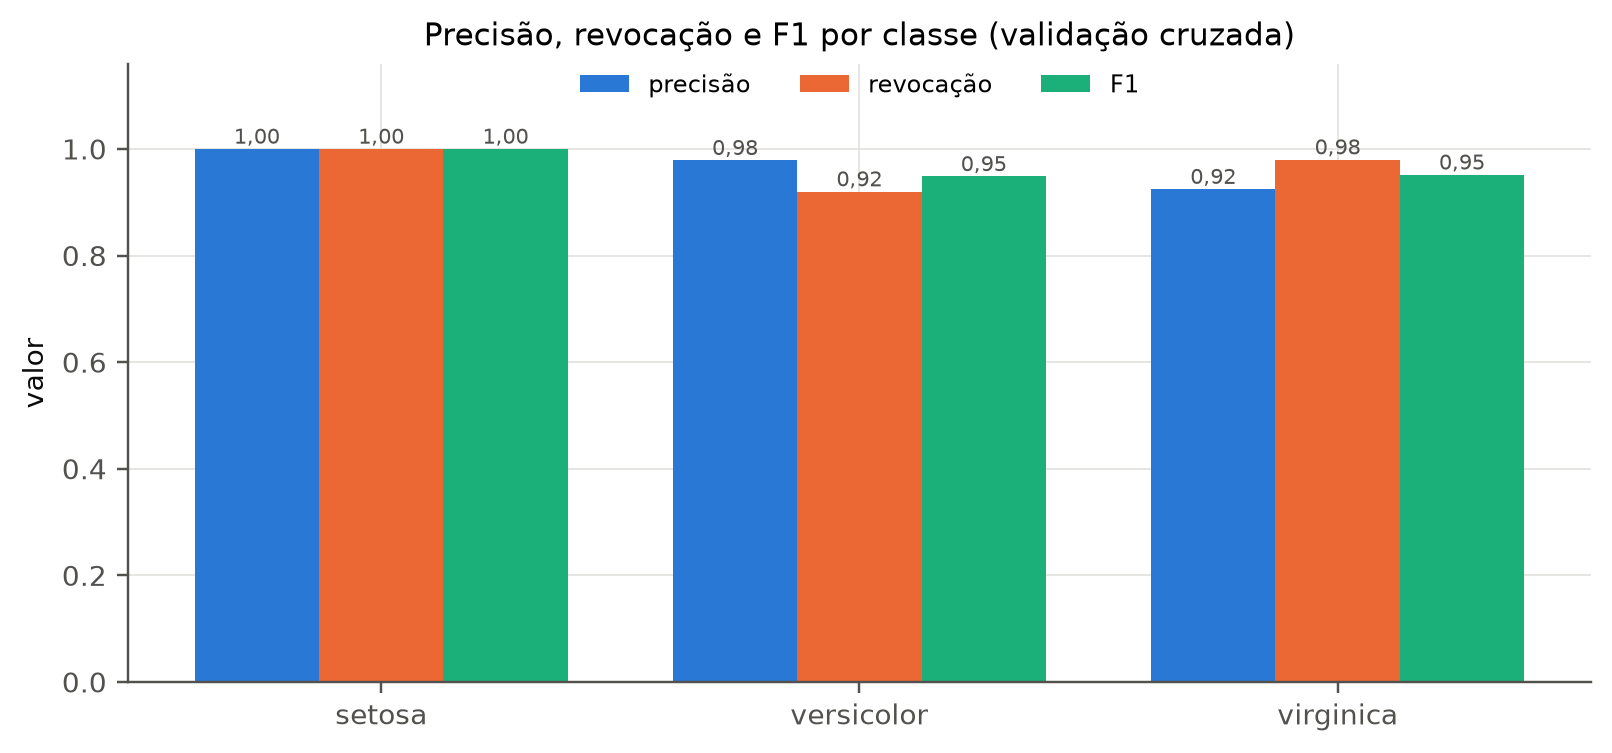
\includegraphics[width=0.78\textwidth]{fig_metricas_por_classe.png}
	\caption{Precisão, revocação e $F_1$ por classe na validação cruzada. O padrão assimétrico
	entre \emph{versicolor} e \emph{virginica} reflete a sobreposição das distribuições na
	fronteira.}
	\label{fig:metricas-classe}
\end{figure}

O padrão é coerente com a \figura{fig:dispersao}: as \emph{versicolor} com pétalas maiores
invadem a região da \emph{virginica}, e a rede, ao tentar separá-las, desloca a fronteira na
direção da \emph{versicolor}, errando mais para o lado da classe maior.

\subsection{Curva de treinamento}

A \figura{fig:curva-perda} mostra a evolução da perda e da acurácia de validação ao longo das
épocas, para o modelo treinado nos \nTreino{} exemplos. A perda cai de forma monotônica e suave,
sem oscilações bruscas --- sinal de que a taxa de aprendizado do Adam está adequada. A acurácia de
validação atinge $90{,}5\,\%$ e estagna; a parada antecipada interrompe o treinamento na época
\nIter{}, devolvendo os pesos da melhor época. A perda final é \perdaFinal{}.

\begin{figure}[htbp]
	\centering
	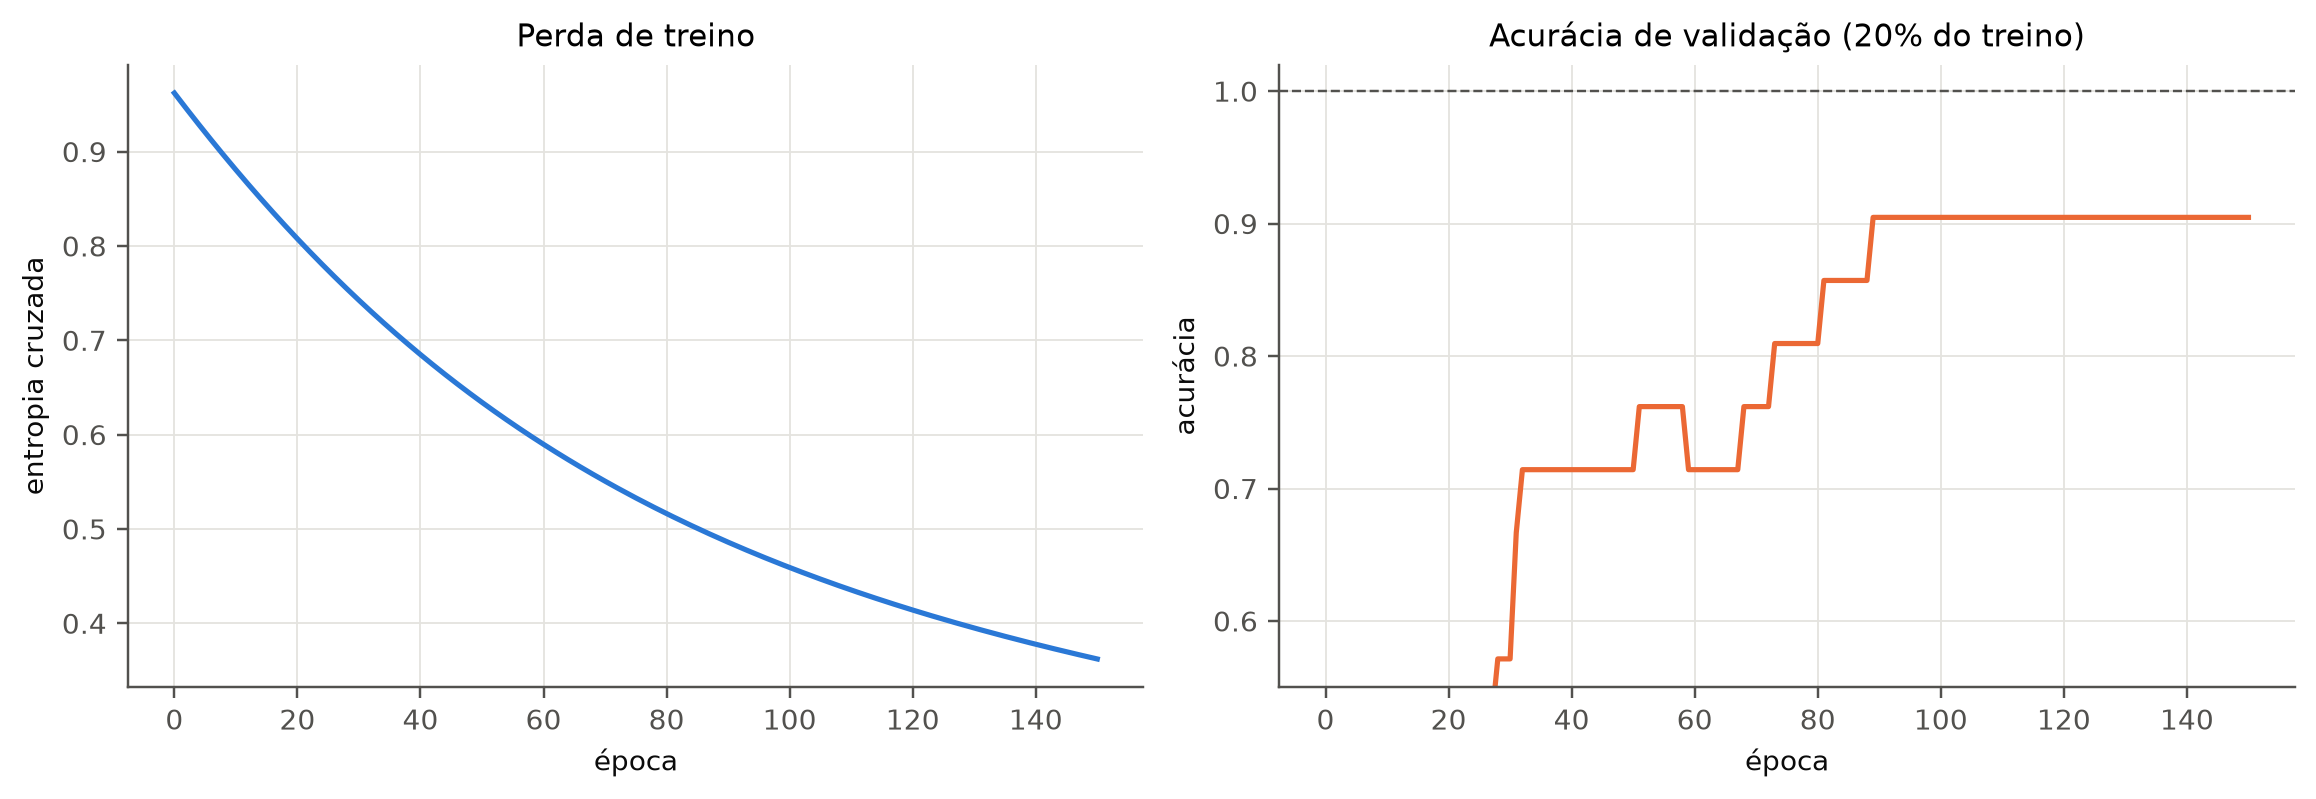
\includegraphics[width=\textwidth]{fig_curva_perda.png}
	\caption{Curva de treinamento: perda de treino (esquerda) e acurácia no conjunto de validação
	interno, 20\,\% do treino (direita). A linha tracejada marca $100\,\%$ de acerto.}
	\label{fig:curva-perda}
\end{figure}

Vale notar que a acurácia de validação interna é mais baixa que a acurácia de teste. Isso não é
paradoxo: o conjunto de validação interno tem apenas 21 amostras, e cada erro custa $4{,}8$ pontos
percentuais. A curva é útil para detectar overfitting e escolher a época de parada, não para
estimar o desempenho final.

\subsection{Curva de aprendizado}

A curva de aprendizado responde a uma pergunta prática: mais dados ajudariam? A
\figura{fig:curva-aprendizado} mostra a acurácia de treino e de validação em função do tamanho do
conjunto de treinamento, mantendo o teste fixo em uma dobra de cada vez.

\begin{figure}[htbp]
	\centering
	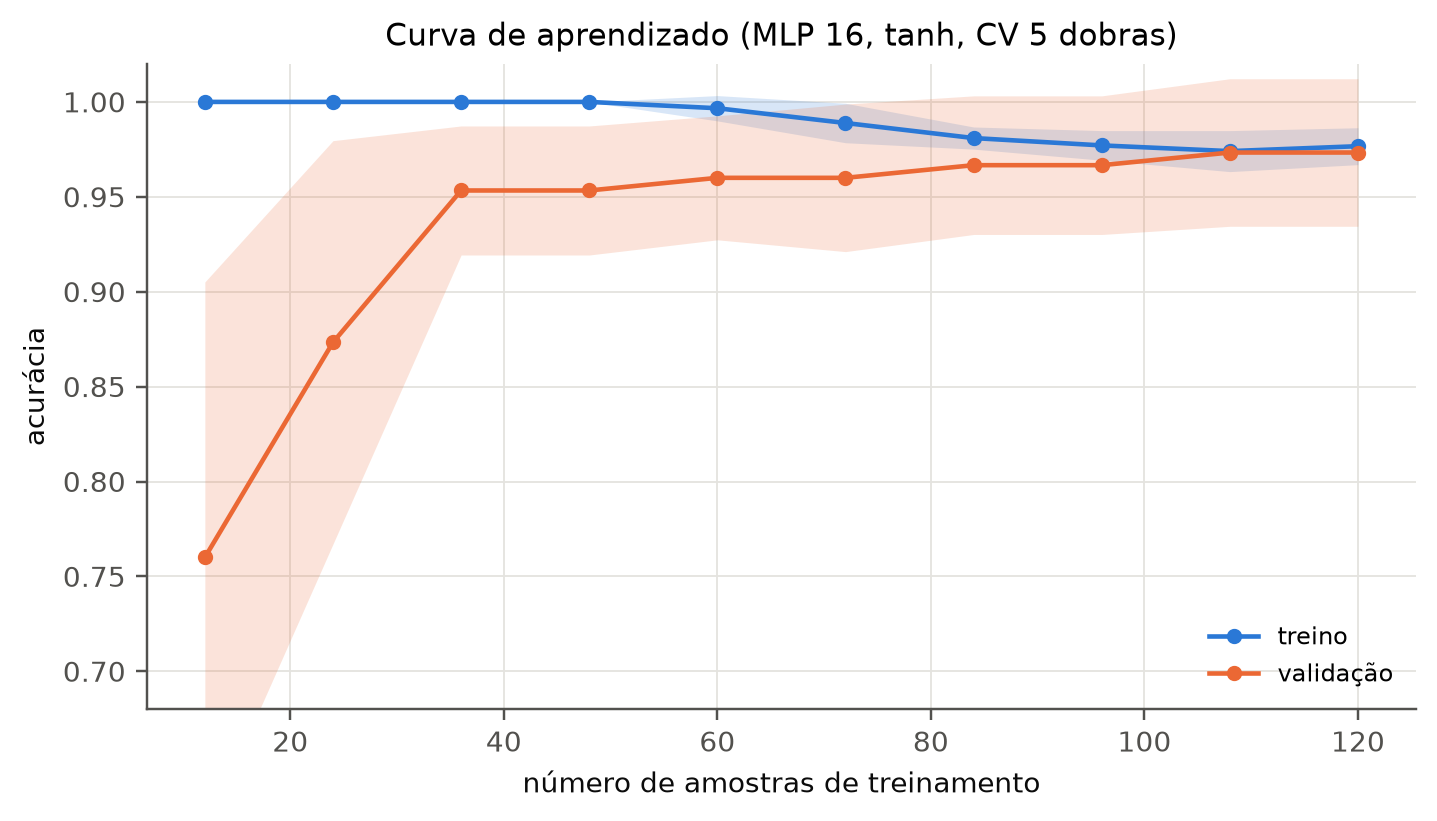
\includegraphics[width=0.78\textwidth]{fig_curva_aprendizado.png}
	\caption{Curva de aprendizado do modelo principal (validação cruzada de 5 dobras, 10 tamanhos
	de treino). A faixa sombreada representa $\pm 1$ desvio-padrão entre as dobras.}
	\label{fig:curva-aprendizado}
\end{figure}

Com 12 amostras de treino, a acurácia de validação é de apenas $76\,\%$ e a variabilidade é enorme.
Com 36 amostras, já chega a $95\,\%$. A partir daí, o ganho é marginal: com 120 amostras, a
validação chega a $97{,}3\,\%$. A curva de treino, por sua vez, cai ligeiramente de $100\,\%$ para
$97{,}7\,\%$ --- a rede deixa de decorar e passa a generalizar. O padrão indica que o problema está
mais limitado pela fronteira entre as classes do que pela quantidade de dados: a partir de ~40
amostras por classe, o retorno de coletar mais dados é pequeno.

\subsection{Efeito da arquitetura}

A \tabela{tab:arquiteturas} e a \figura{fig:arquiteturas} comparam nove arquiteturas, de um único
neurônio a duas camadas com $128$ e $64$ neurônios. O resultado é inequívoco: \emph{a arquitetura
quase não importa neste problema}. Todas as configurações ficam entre $94{,}7\,\%$ e
$96{,}7\,\%$, uma faixa de 2 pontos percentuais, enquanto o desvio entre dobras é de cerca de
$4$ pontos.

\begin{table}[htbp]
	\centering
	\caption{Acurácia por arquitetura (validação cruzada 5 dobras $\times$ 3 repetições). A coluna
	de parâmetros conta pesos e vieses.}
	\label{tab:arquiteturas}
	% gerado automaticamente por mlp_iris.py - nao editar

\begin{tabular}{lrrrrr}
\toprule
\textbf{arquitetura} & \textbf{profundidade} & \textbf{parâmetros} & \textbf{acurácia} & \textbf{desvio} & \textbf{log-loss} \\
\midrule
(4) & 1 & 35 & 96{,}7 & 4{,}0 & 0{,}171 \\
(8) & 1 & 67 & 95{,}3 & 3{,}5 & 0{,}112 \\
(16) & 1 & 131 & 94{,}7 & 4{,}1 & 0{,}104 \\
(32) & 1 & 259 & 94{,}9 & 4{,}0 & 0{,}103 \\
(8, 4) & 2 & 91 & 96{,}2 & 3{,}3 & 0{,}083 \\
(16, 8) & 2 & 243 & 95{,}3 & 3{,}7 & 0{,}096 \\
(32, 16) & 2 & 739 & 94{,}7 & 4{,}1 & 0{,}095 \\
(64, 32) & 2 & 2499 & 95{,}3 & 4{,}3 & 0{,}102 \\
(128, 64) & 2 & 9091 & 94{,}9 & 4{,}5 & 0{,}154 \\
\bottomrule
\end{tabular}

\end{table}

\begin{figure}[htbp]
	\centering
	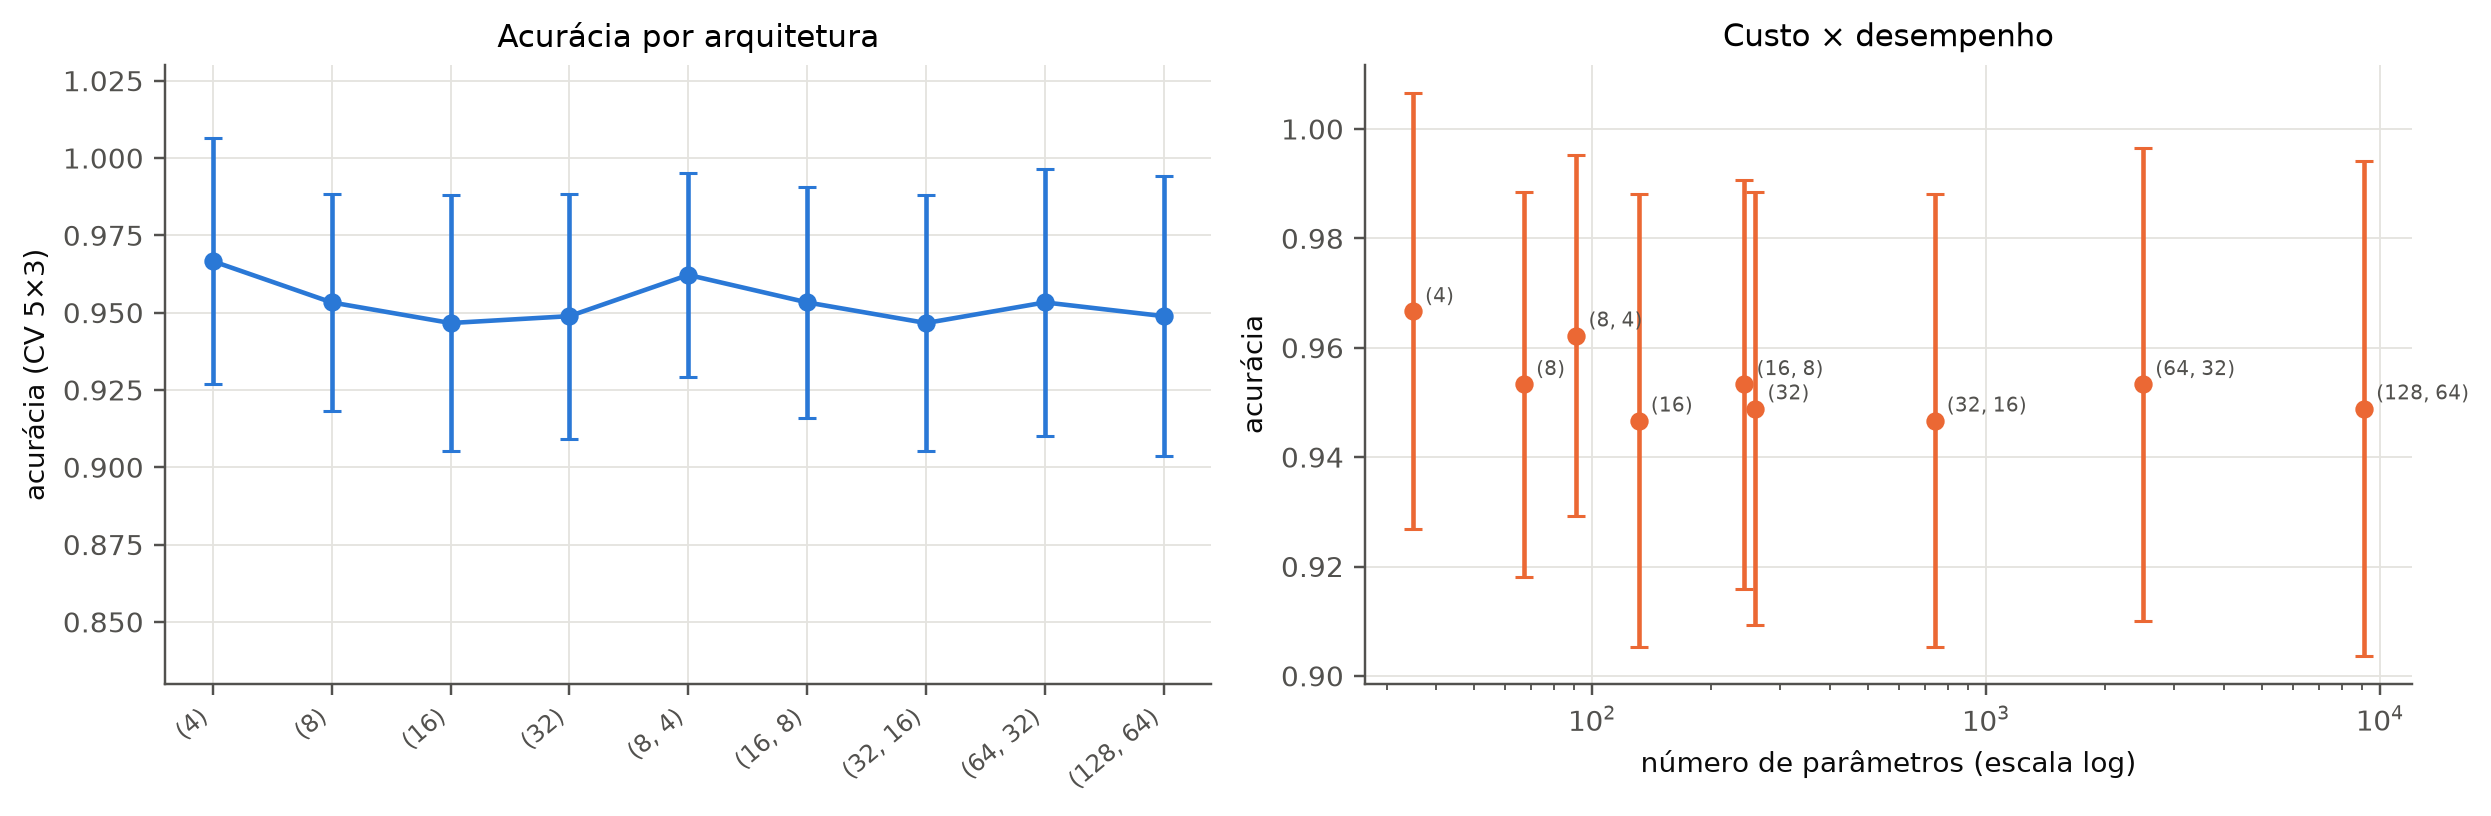
\includegraphics[width=\textwidth]{fig_arquiteturas.png}
	\caption{Acurácia por arquitetura (esquerda) e relação entre número de parâmetros e acurácia
	(direita, escala logarítmica). As barras de erro são $\pm 1$ desvio-padrão entre as 15 dobras.}
	\label{fig:arquiteturas}
\end{figure}

Dois pontos merecem comentário. Primeiro, a melhor configuração é a menor: um único neurônio
oculto com 4 unidades ($96{,}7\,\%$, 35 parâmetros). Segundo, as redes maiores não melhoram ---
pioram ligeiramente. A rede com $128$ e $64$ neurônios tem 9\,091 parâmetros para 150 amostras,
uma razão de 60 parâmetros por amostra, e sua acurácia cai para $94{,}9\,\%$ com o maior desvio de
todas as configurações. É o retrato clássico do excesso de capacidade: o modelo tem liberdade para
ajustar ruído.

Esse resultado não significa que arquiteturas maiores sejam inúteis; significa que, \emph{neste
problema}, a informação está em duas dimensões efetivas e uma fronteira simples basta. A
\figura{fig:fronteira-capacidade} mostra exatamente isso: as fronteiras de decisão de redes com 2,
4, 24 e 112 neurônios são visualmente quase idênticas.

\subsection{Efeito da função de ativação}

A \tabela{tab:ativacoes} compara quatro ativações com a mesma arquitetura $(16,8)$. A
\emph{tanh} e a logística lideram ($96{,}2\,\%$), a ReLU fica em $95{,}3\,\%$ e a identidade em
$96{,}0\,\%$. As diferenças estão dentro de um desvio-padrão e não devem ser interpretadas como
superioridade de uma função sobre outra.

\begin{table}[htbp]
	\centering
	\caption{Efeito da função de ativação na camada oculta (arquitetura $(16,8)$,
	validação cruzada 5 $\times$ 3).}
	\label{tab:ativacoes}
	% gerado automaticamente por mlp_iris.py - nao editar

\begin{tabular}{lrrr}
\toprule
\textbf{ativação} & \textbf{acurácia} & \textbf{desvio} & \textbf{log-loss} \\
\midrule
relu & 95{,}3 & 3{,}7 & 0{,}096 \\
tanh & 96{,}2 & 3{,}3 & 0{,}095 \\
logistic & 96{,}2 & 3{,}3 & 0{,}106 \\
identity & 96{,}0 & 3{,}4 & 0{,}083 \\
\bottomrule
\end{tabular}

\end{table}

\begin{figure}[htbp]
	\centering
	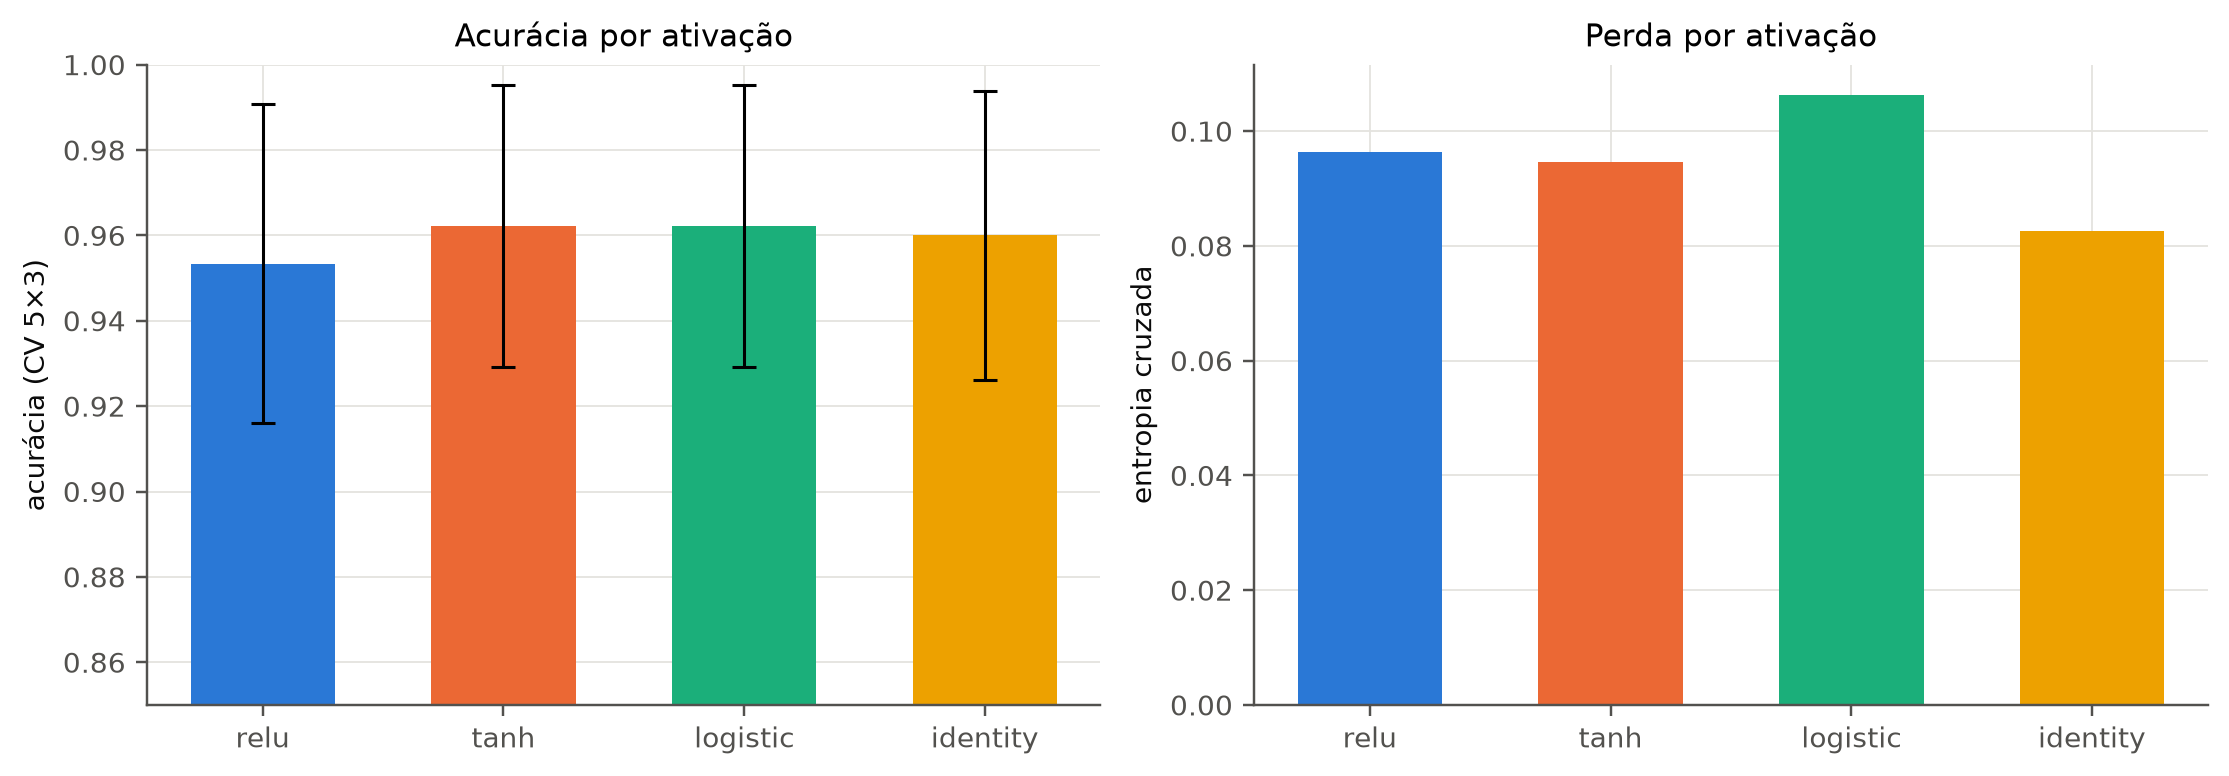
\includegraphics[width=\textwidth]{fig_ativacoes.png}
	\caption{Acurácia e entropia cruzada por função de ativação. A identidade, que torna a rede
	um modelo linear, tem a menor entropia cruzada --- evidência de que o problema é quase
	linearmente separável.}
	\label{fig:ativacoes}
\end{figure}

O detalhe mais informativo está na coluna de entropia cruzada: a \emph{identidade} tem a menor
perda ($0{,}083$), seguida de perto por \emph{tanh} ($0{,}095$) e ReLU ($0{,}096$). Uma rede sem
não linearidade na camada oculta produz a melhor calibração de probabilidades. Isso é uma pista
forte de que a fronteira entre as classes é essencialmente linear e que a não linearidade não está
sendo usada para melhorar a separação --- apenas para ajustar detalhes.

\subsection{Efeito da regularização}

A \figura{fig:regularizacao} varre $\alpha$ de $10^{-6}$ a $10^{2}$ em escala logarítmica, com a
arquitetura $(32,16)$. O comportamento tem três regimes bem definidos:

\begin{itemize}
	\item \textbf{$\alpha \lesssim 1$}: acurácia praticamente constante em torno de $95$--$96\,\%$ e
	      entropia cruzada mínima. A regularização é fraca demais para ter efeito;
	\item \textbf{$\alpha \approx 1$}: a entropia cruzada atinge o mínimo ($0{,}089$). É o ponto em
	      que a penalidade começa a estabilizar as probabilidades;
	\item \textbf{$\alpha \gtrsim 10$}: colapso. Com $\alpha = 10$, a acurácia cai para
	      $89\,\%$; com $\alpha = 100$, para $33\,\%$ --- o modelo prevê uma única classe para
	      todas as amostras, porque a penalidade domina a perda e os pesos vão a zero.
\end{itemize}

\begin{figure}[htbp]
	\centering
	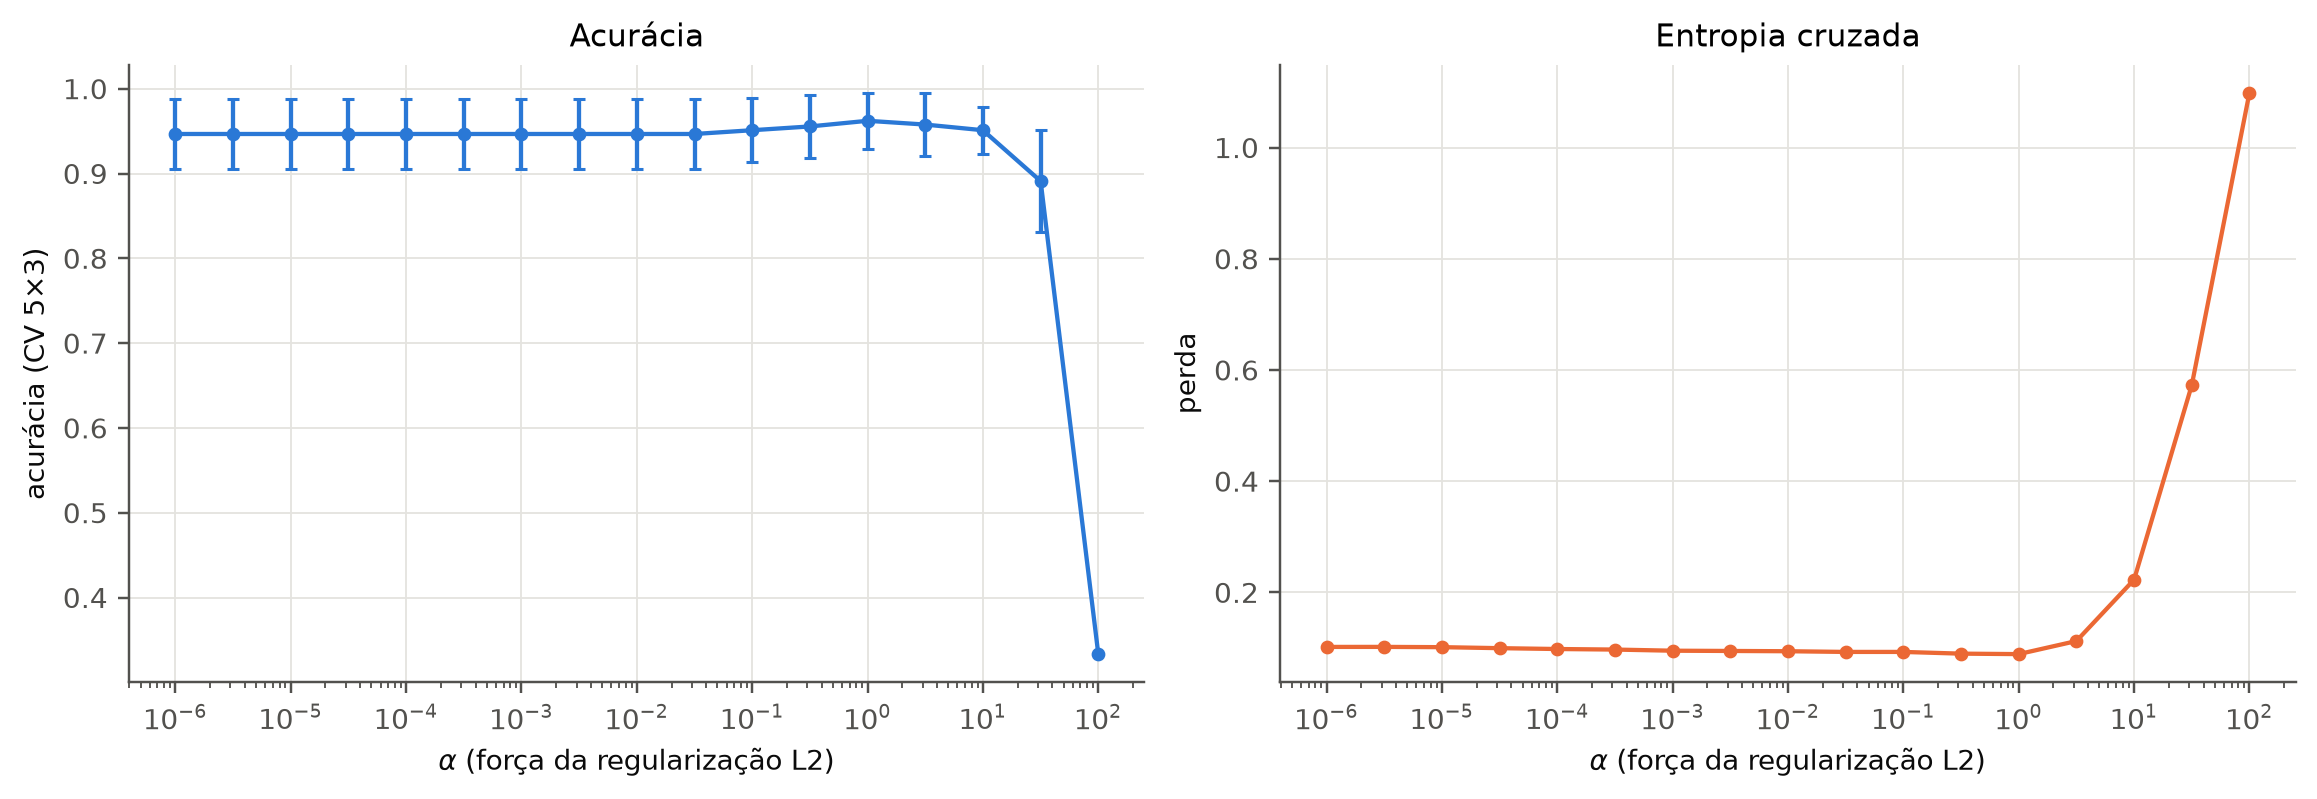
\includegraphics[width=\textwidth]{fig_regularizacao.png}
	\caption{Efeito da força de regularização $L_2$ na acurácia e na entropia cruzada
	(arquitetura $(32,16)$, validação cruzada 5 $\times$ 3).}
	\label{fig:regularizacao}
\end{figure}

A lição prática é que existe uma faixa larga de valores seguros e um penhasco abrupto. Para um
problema pequeno como o Iris, qualquer $\alpha$ entre $10^{-4}$ e $10^{-1}$ funciona; a escolha de
$10^{-2}$ está confortavelmente no meio dessa faixa.

\subsection{Efeito da taxa de aprendizado}

A \figura{fig:taxas} mostra o treinamento com SGD e momento para cinco taxas iniciais. Os
resultados resumem o que se espera de um otimizador de primeira ordem:

\begin{itemize}
	\item $\eta_0 = 10^{-3}$: a perda mal se move em 300 épocas ($0{,}73$) e a acurácia de treino
	      fica em $68\,\%$. A taxa é pequena demais;
	\item $\eta_0 = 10^{-2}$: convergência lenta, mas estável ($0{,}082$);
	\item $\eta_0 = 5\times10^{-2}$ e $10^{-1}$: convergência rápida e perda final baixa
	      ($0{,}041$ e $0{,}039$), com acurácia de treino de $98{,}7\,\%$;
	\item $\eta_0 = 5\times10^{-1}$: a perda despenca e depois oscila; a acurácia final cai para
	      $98\,\%$. A taxa é grande demais e o otimizador não se estabiliza.
\end{itemize}

\begin{figure}[htbp]
	\centering
	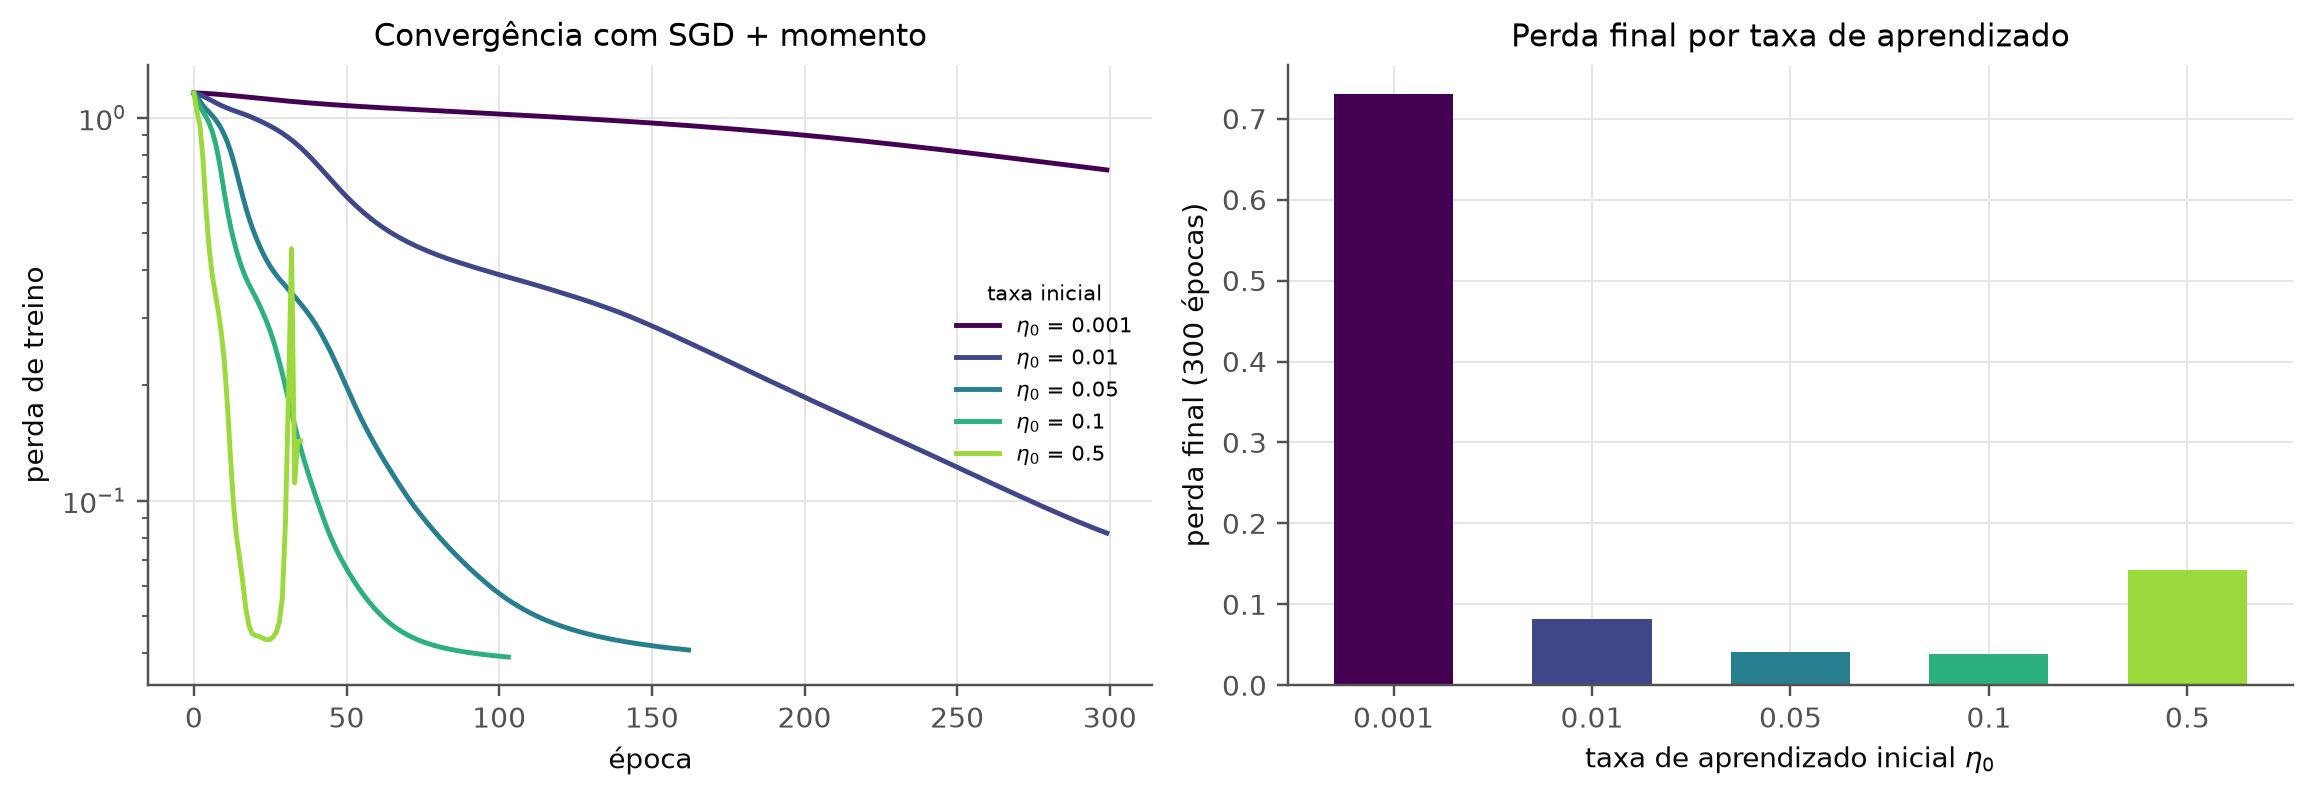
\includegraphics[width=\textwidth]{fig_taxas_aprendizado.png}
	\caption{Convergência do SGD com momento para diferentes taxas iniciais. À esquerda, perda de
	treino em escala logarítmica; à direita, perda final após 300 épocas.}
	\label{fig:taxas}
\end{figure}

A faixa útil vai de $10^{-2}$ a $10^{-1}$. O Adam, usado no modelo final, é mais tolerante: por
normalizar o passo por parâmetro, aceita taxas maiores sem divergir, e o padrão $10^{-3}$ do
scikit-learn foi suficiente.

\subsection{Fronteiras de decisão}

Para visualizar o que a rede aprendeu, a \figura{fig:fronteira-comparacao} treina quatro modelos
usando apenas comprimento e largura da pétala --- as duas variáveis mais informativas --- e mostra
as regiões de decisão no plano.

\begin{figure}[htbp]
	\centering
	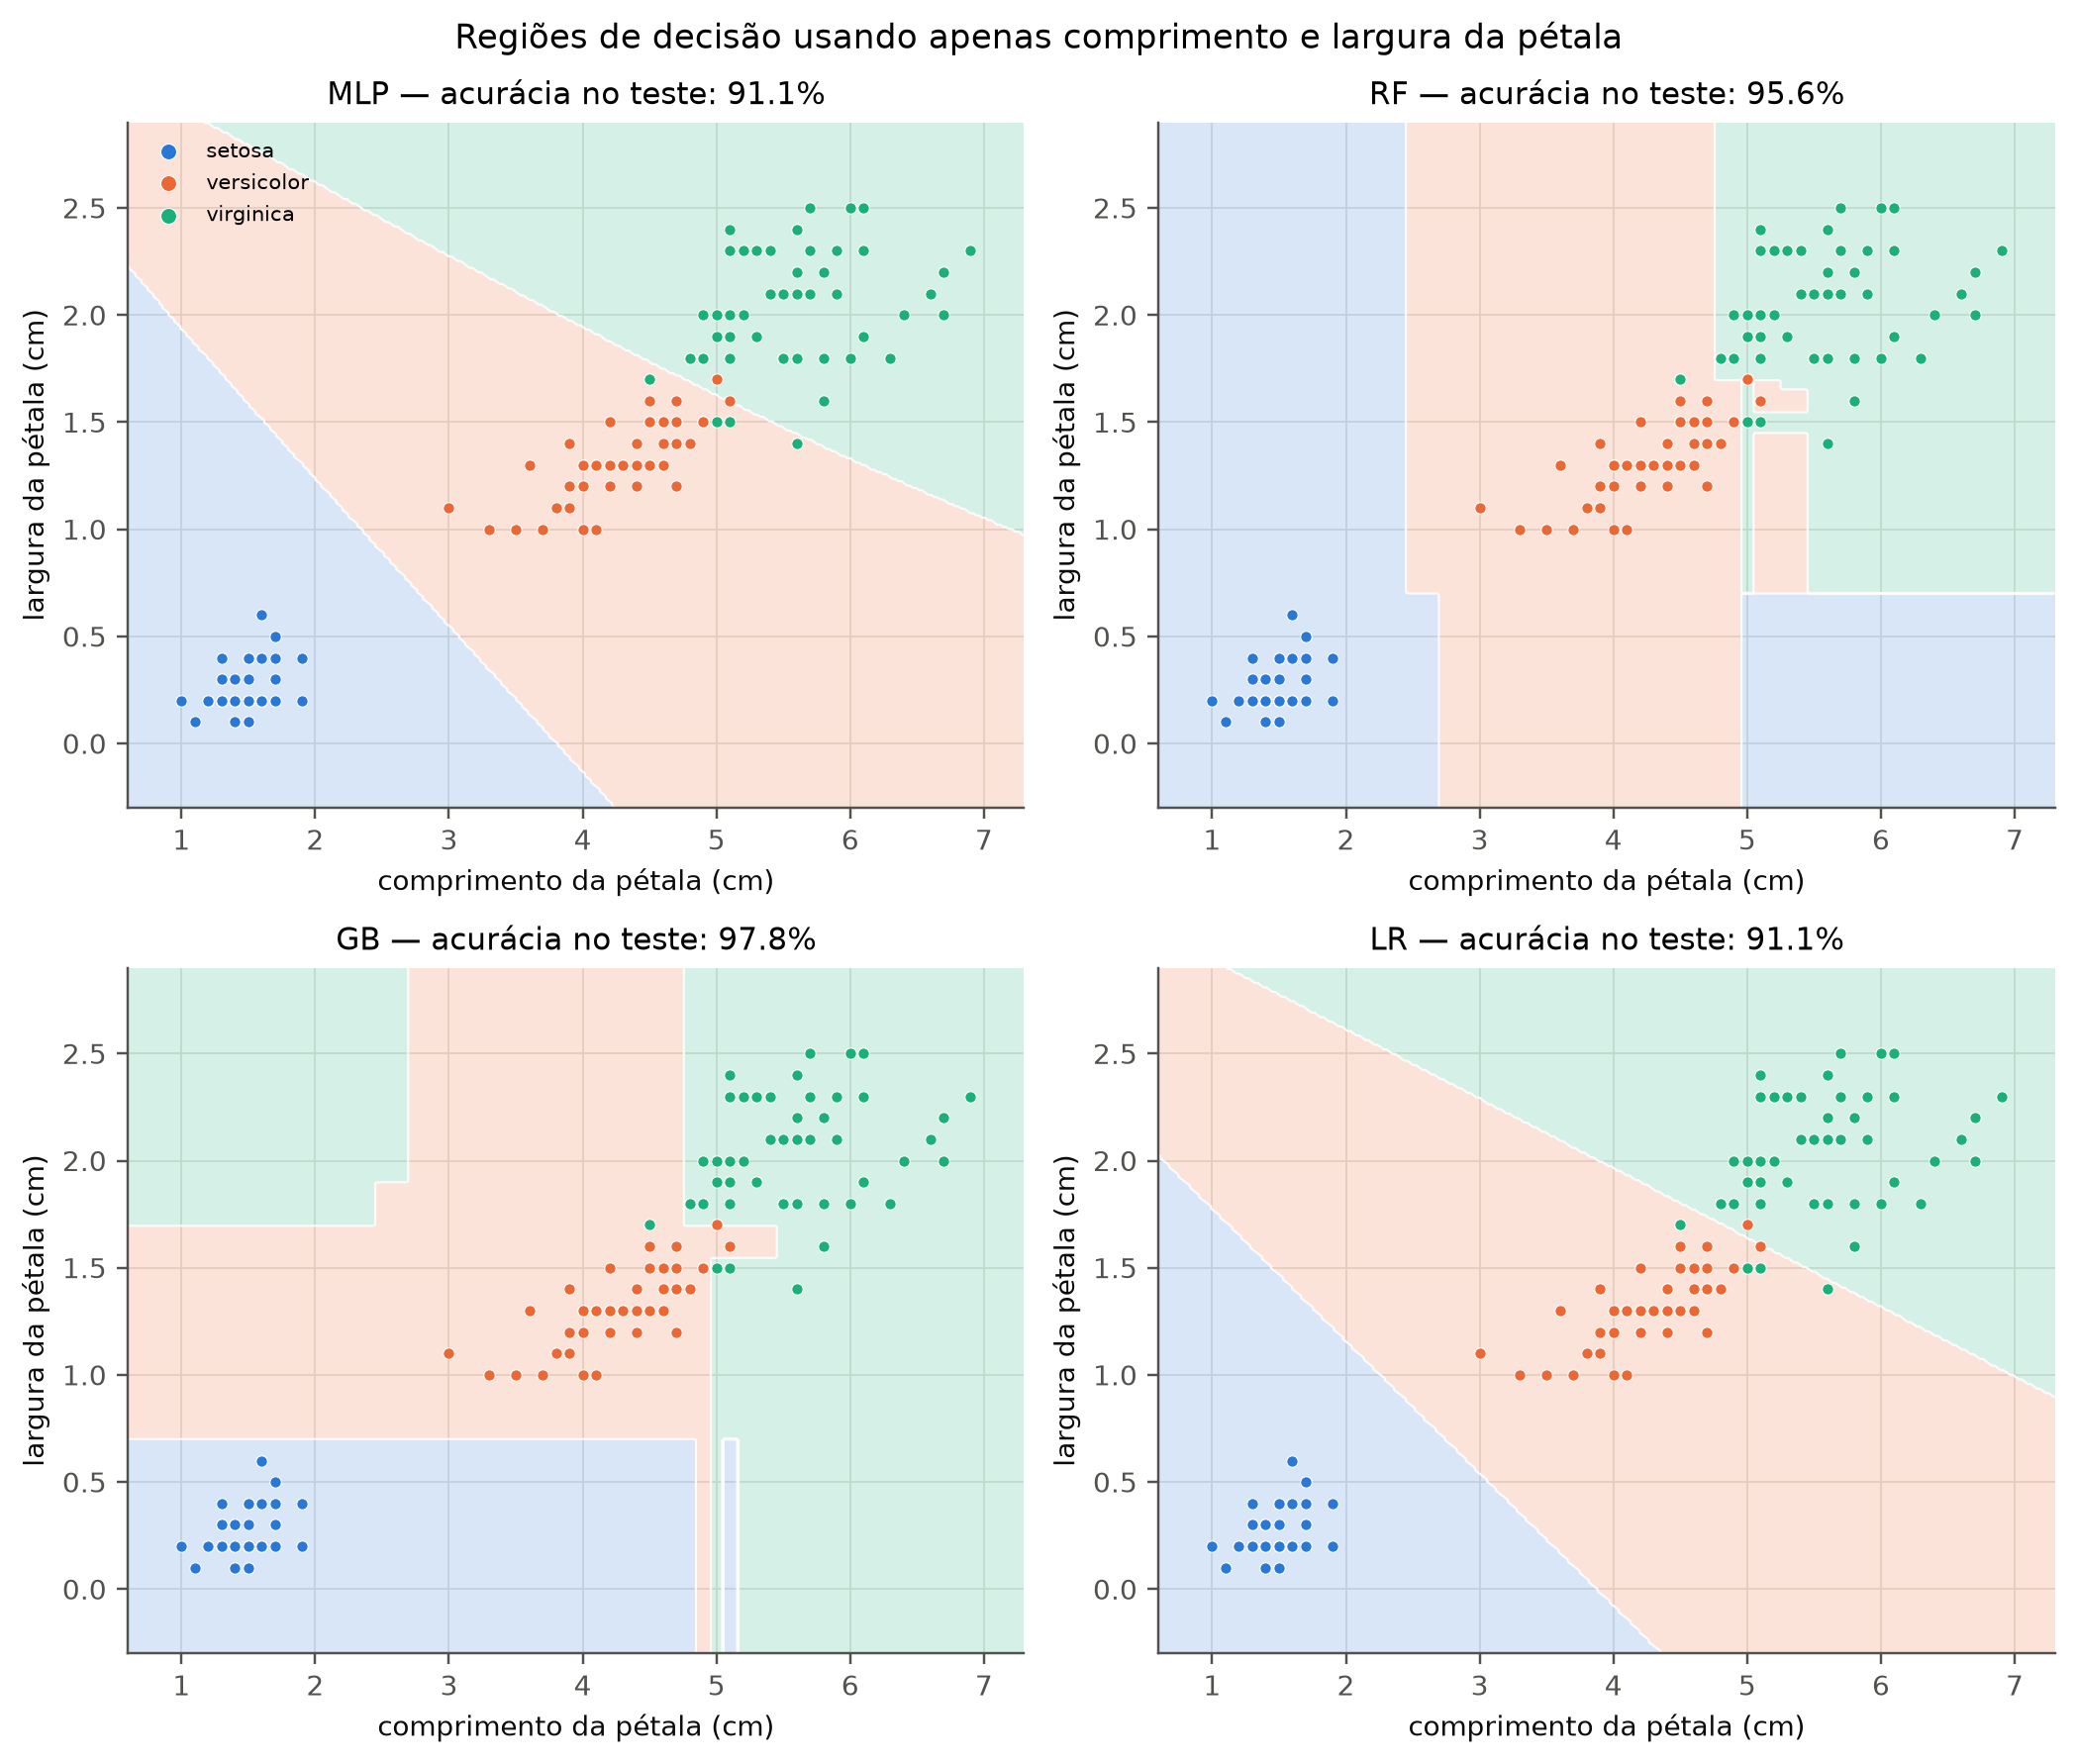
\includegraphics[width=0.95\textwidth]{fig_fronteira_comparacao.png}
	\caption{Regiões de decisão no plano da pétala para MLP, floresta aleatória, \emph{gradient
	boosting} e regressão logística. Cada modelo foi treinado apenas com os dois atributos
	mostrados; a acurácia indicada é a do conjunto de teste com esses dois atributos.}
	\label{fig:fronteira-comparacao}
\end{figure}

O resultado é revelador. A MLP produz duas fronteiras praticamente retas, assim como a regressão
logística. A floresta aleatória produz uma escada de retângulos, e o \emph{gradient boosting}
produz uma fronteira irregular que se ajusta a pontos individuais. Apesar das formas tão
diferentes, as acurácias são próximas: $91{,}1\,\%$ para MLP e regressão logística,
$95{,}6\,\%$ para a floresta e $97{,}8\,\%$ para o \emph{boosting}.

A semelhança entre MLP e regressão logística é a confirmação visual do que a entropia cruzada da
\tabela{tab:ativacoes} já sugeria: com duas variáveis e classes quase separáveis por uma reta, a
não linearidade da rede não encontra estrutura curva para explorar.

A \figura{fig:fronteira-capacidade} repete o exercício para redes de capacidade crescente. Mesmo
com 112 neurônios em três camadas, a fronteira permanece quase linear. A rede tem capacidade para
curvas muito mais complexas, mas os dados não pedem isso --- e a regularização $L_2$ desencoraja o
ajuste fino.

\begin{figure}[htbp]
	\centering
	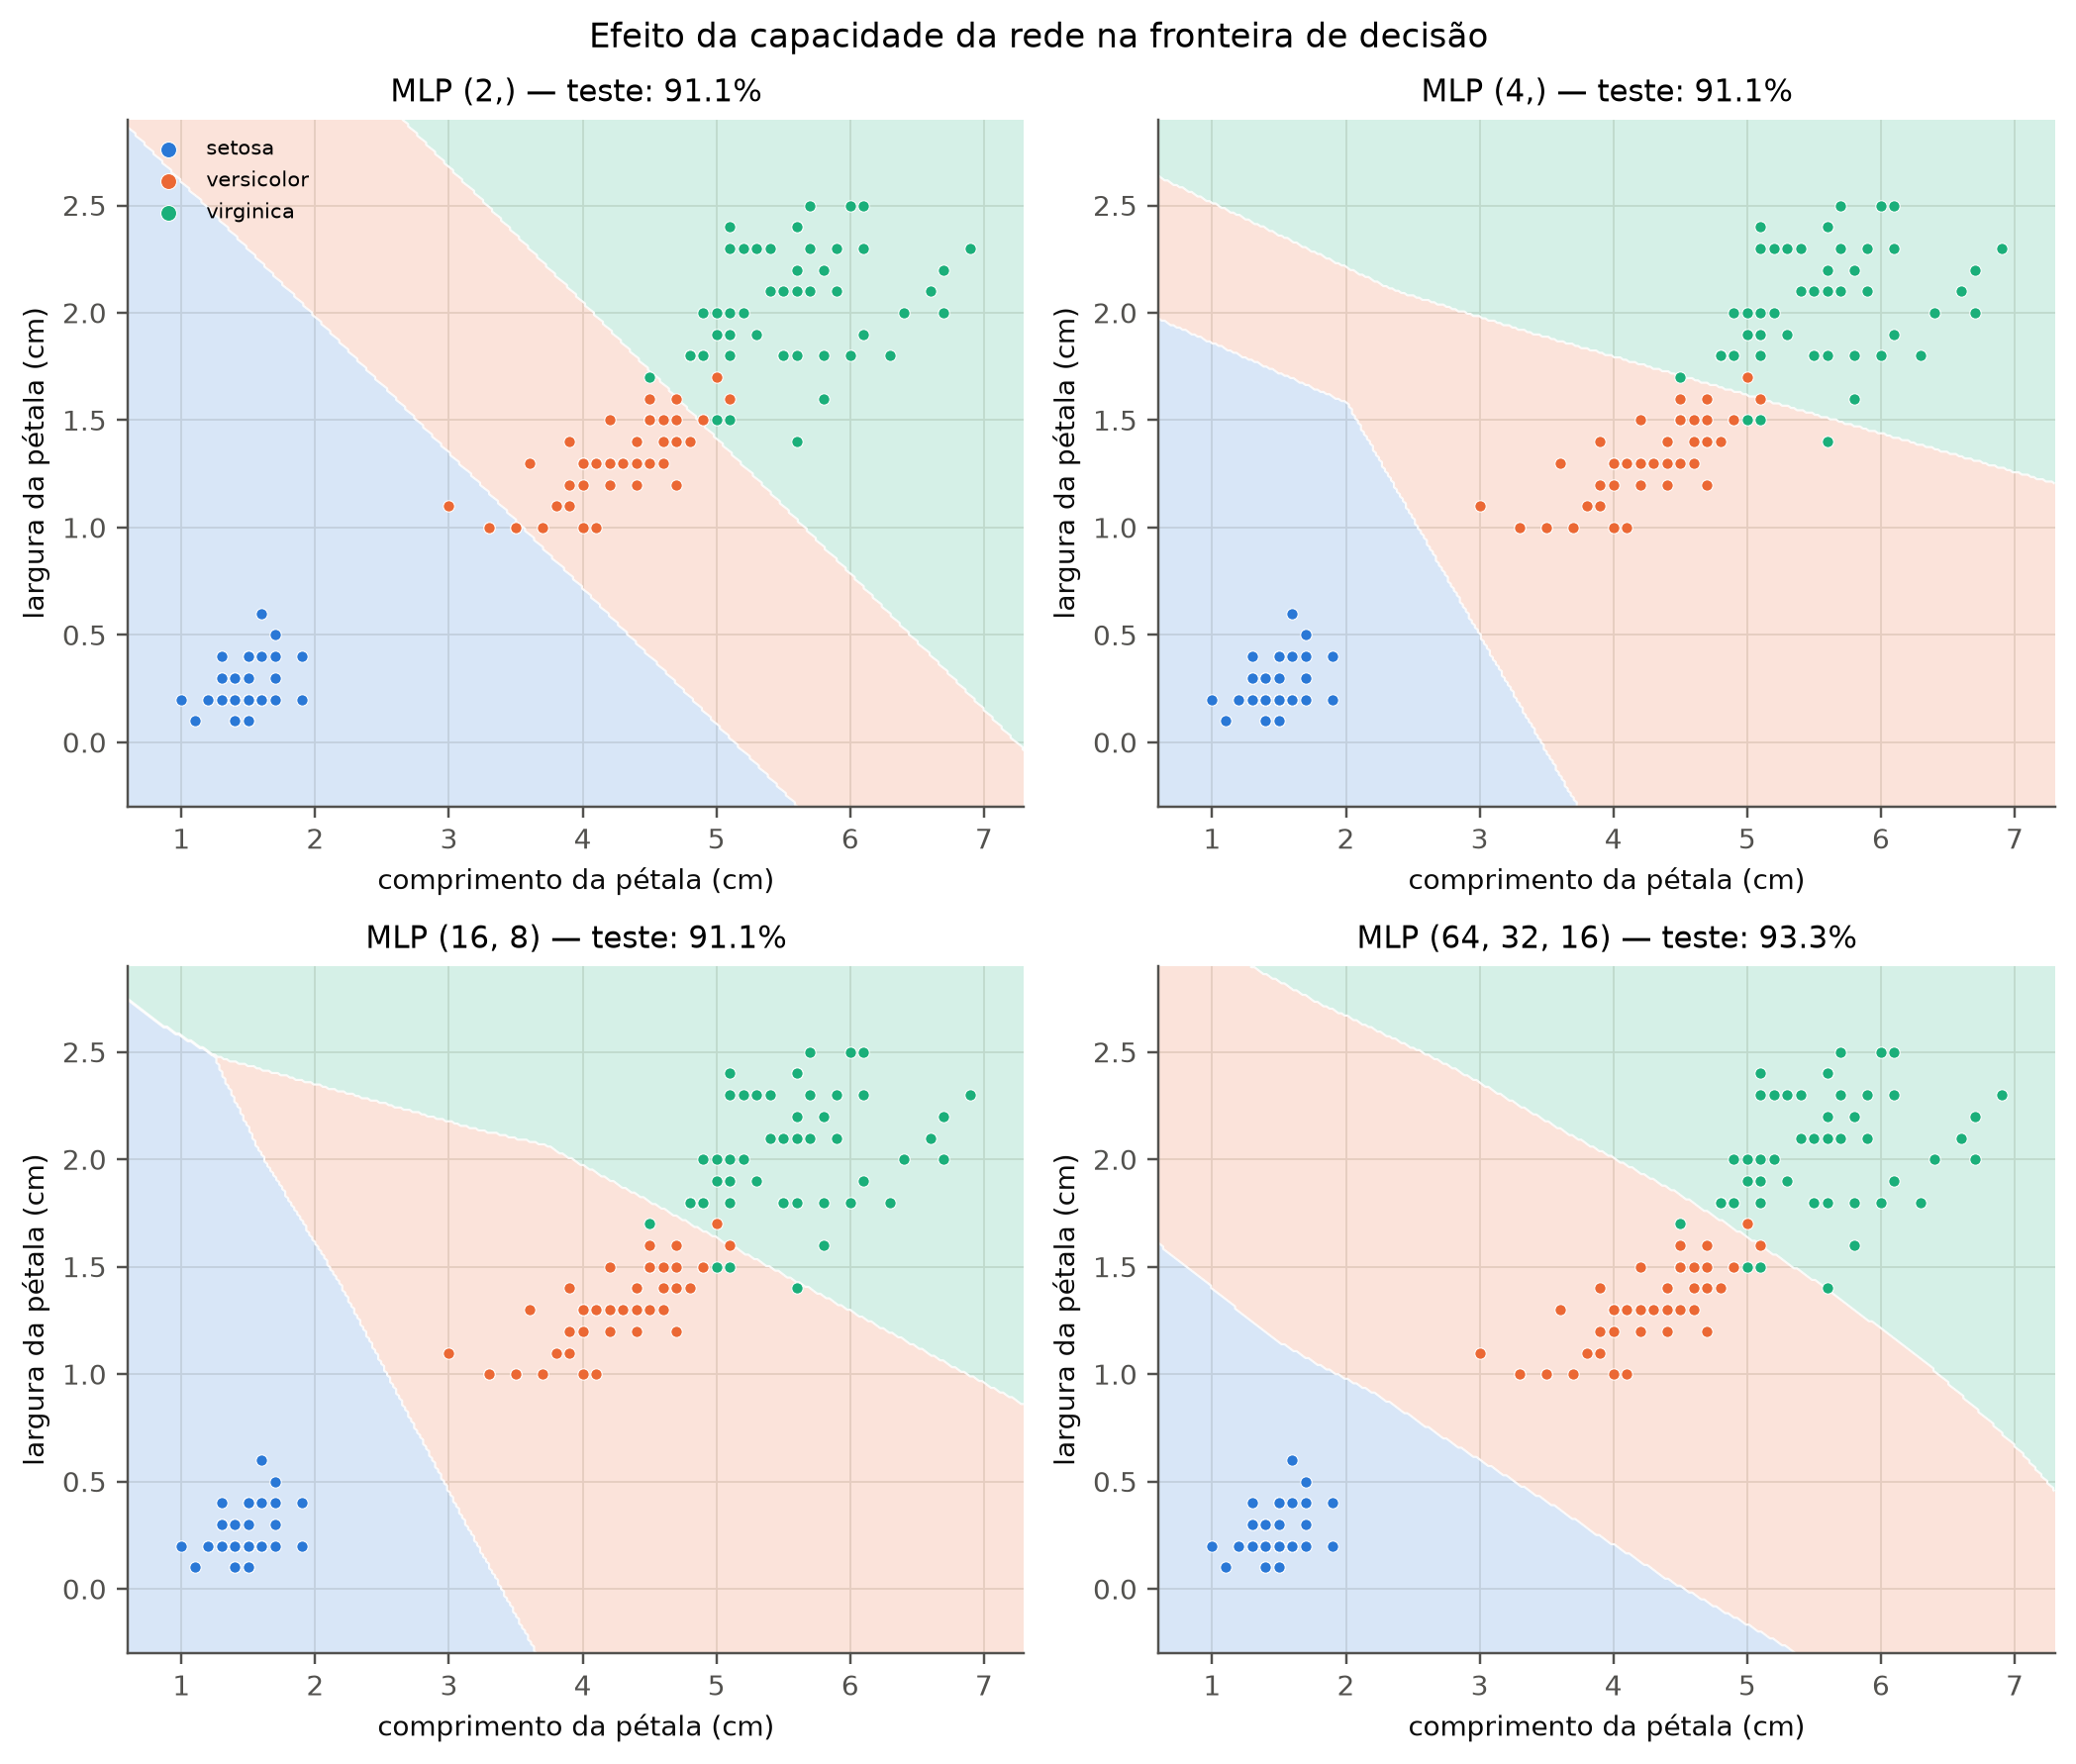
\includegraphics[width=0.95\textwidth]{fig_fronteira_capacidade.png}
	\caption{Fronteira de decisão para quatro capacidades, com os mesmos dois atributos. O aumento
	da capacidade não produz fronteiras mais complexas porque o problema é quase linearmente
	separável.}
	\label{fig:fronteira-capacidade}
\end{figure}

\subsection{Importância dos atributos}

A importância por permutação mede quanto a acurácia cai quando um atributo é embaralhado,
destruindo sua relação com a resposta. A \figura{fig:importancia} mostra o resultado para o
modelo de quatro atributos, no conjunto de teste, com 40 repetições.

\begin{figure}[htbp]
	\centering
	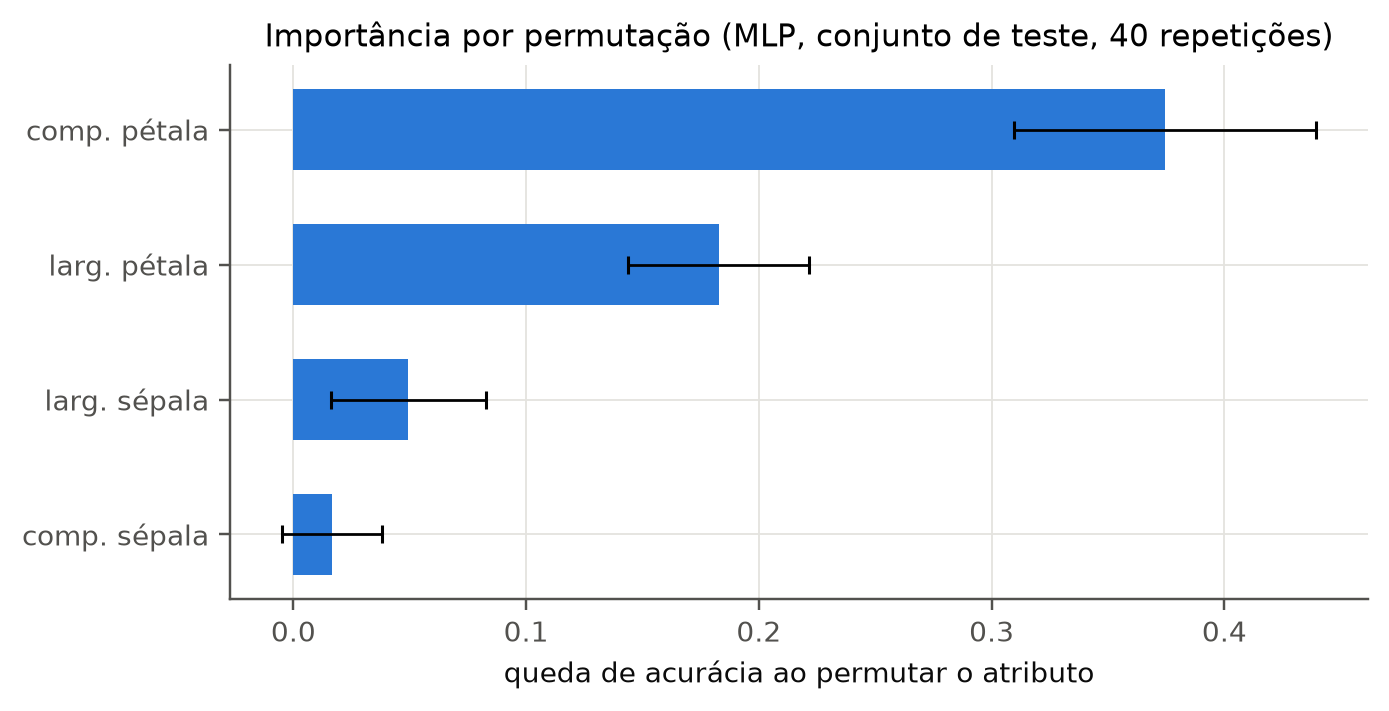
\includegraphics[width=0.72\textwidth]{fig_importancia.png}
	\caption{Importância por permutação no conjunto de teste (MLP de quatro atributos, 40
	repetições). A barra de erro é o desvio-padrão entre repetições.}
	\label{fig:importancia}
\end{figure}

O comprimento da pétala domina, com queda média de $37{,}4$ pontos percentuais. A largura da
pétala vem em segundo lugar ($18{,}3$), seguida pela largura da sépala ($4{,}9$) e pelo
comprimento da sépala ($1{,}7$). A hierarquia coincide com a análise exploratória: a pétala carrega
quase toda a informação discriminante, e a sépala contribui pouco.

Vale registrar uma limitação do método: quando dois atributos são muito correlacionados, permutar
um deles tem efeito pequeno, porque o outro carrega informação semelhante. Comprimento e largura
da pétala têm correlação de $0{,}96$; parte da importância de um é ``emprestada'' do outro. A
conclusão segura é que a pétala é o grupo informativo, não que o comprimento seja exatamente $7$
vezes mais importante que a largura.

\subsection{O que a rede aprendeu}

A \figura{fig:pesos} abre a caixa-preta: mostra as matrizes de pesos de uma rede compacta com 8
neurônios ocultos, treinada em todos os dados.

\begin{figure}[htbp]
	\centering
	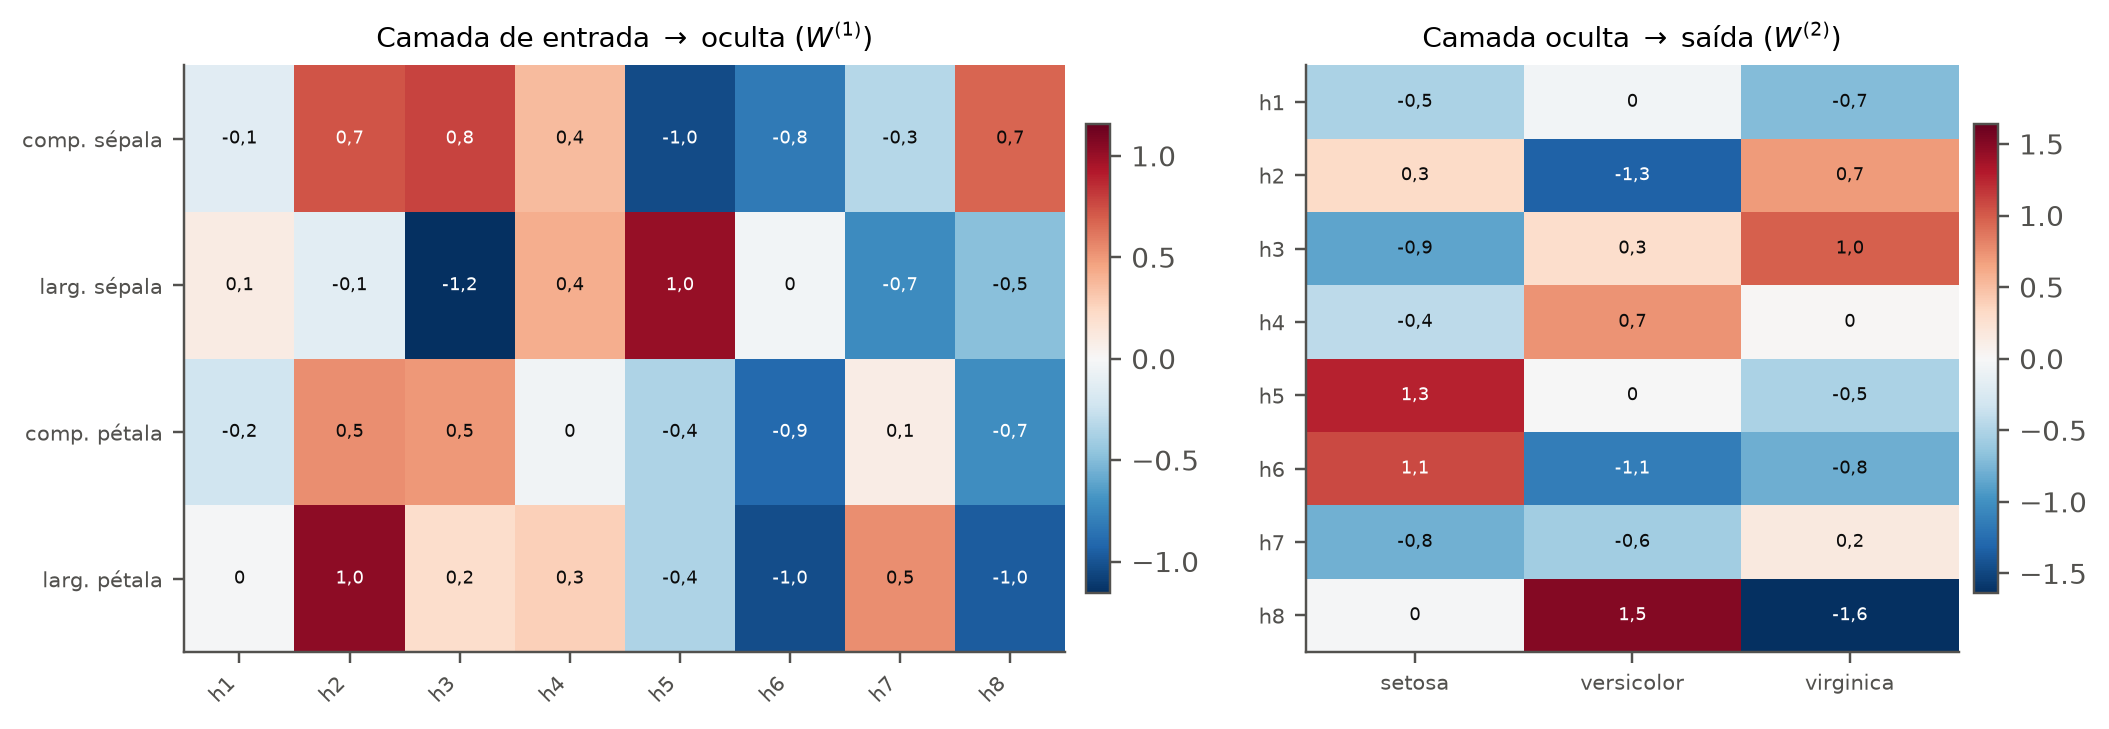
\includegraphics[width=\textwidth]{fig_pesos.png}
	\caption{Pesos aprendidos por uma rede $4$--$8$--$3$. À esquerda, $W^{(1)}$: quanto cada
	atributo pesa em cada neurônio oculto. À direita, $W^{(2)}$: quanto cada neurônio oculto
	contribui para cada classe. Azul é peso negativo, vermelho, positivo.}
	\label{fig:pesos}
\end{figure}

Alguns padrões são interpretáveis. Os neurônios $h_5$ e $h_6$ recebem peso positivo forte da
largura da pétala e do comprimento da pétala, e projetam-se de forma oposta em \emph{setosa} e
\emph{virginica} --- são detectores de ``pétala grande''. O neurônio $h_2$ tem peso positivo no
comprimento da sépala, mas não na pétala, e contribui negativamente para \emph{setosa}: captura a
sépala alongada que caracteriza as espécies maiores. Os demais neurônios combinam atributos de
forma menos óbvia, o que é esperado: a rede distribui a representação por várias unidades
redundantes.

O ponto didático é que a interpretabilidade não é automática. Os pesos são legíveis, mas a
``explicação'' só emerge quando combinados com a análise de importância e com o conhecimento do
problema. Em redes maiores, essa leitura direta deixa de ser viável e recorre-se a métodos
post-hoc.

\subsection{Comparação com modelos de referência}

A \tabela{tab:modelos} e a \figura{fig:comparacao} colocam a MLP ao lado de três alternativas, com
as mesmas dobras: floresta aleatória (400 árvores), \emph{gradient boosting} (300 estimadores) e
regressão logística multinomial.

\begin{figure}[htbp]
	\centering
	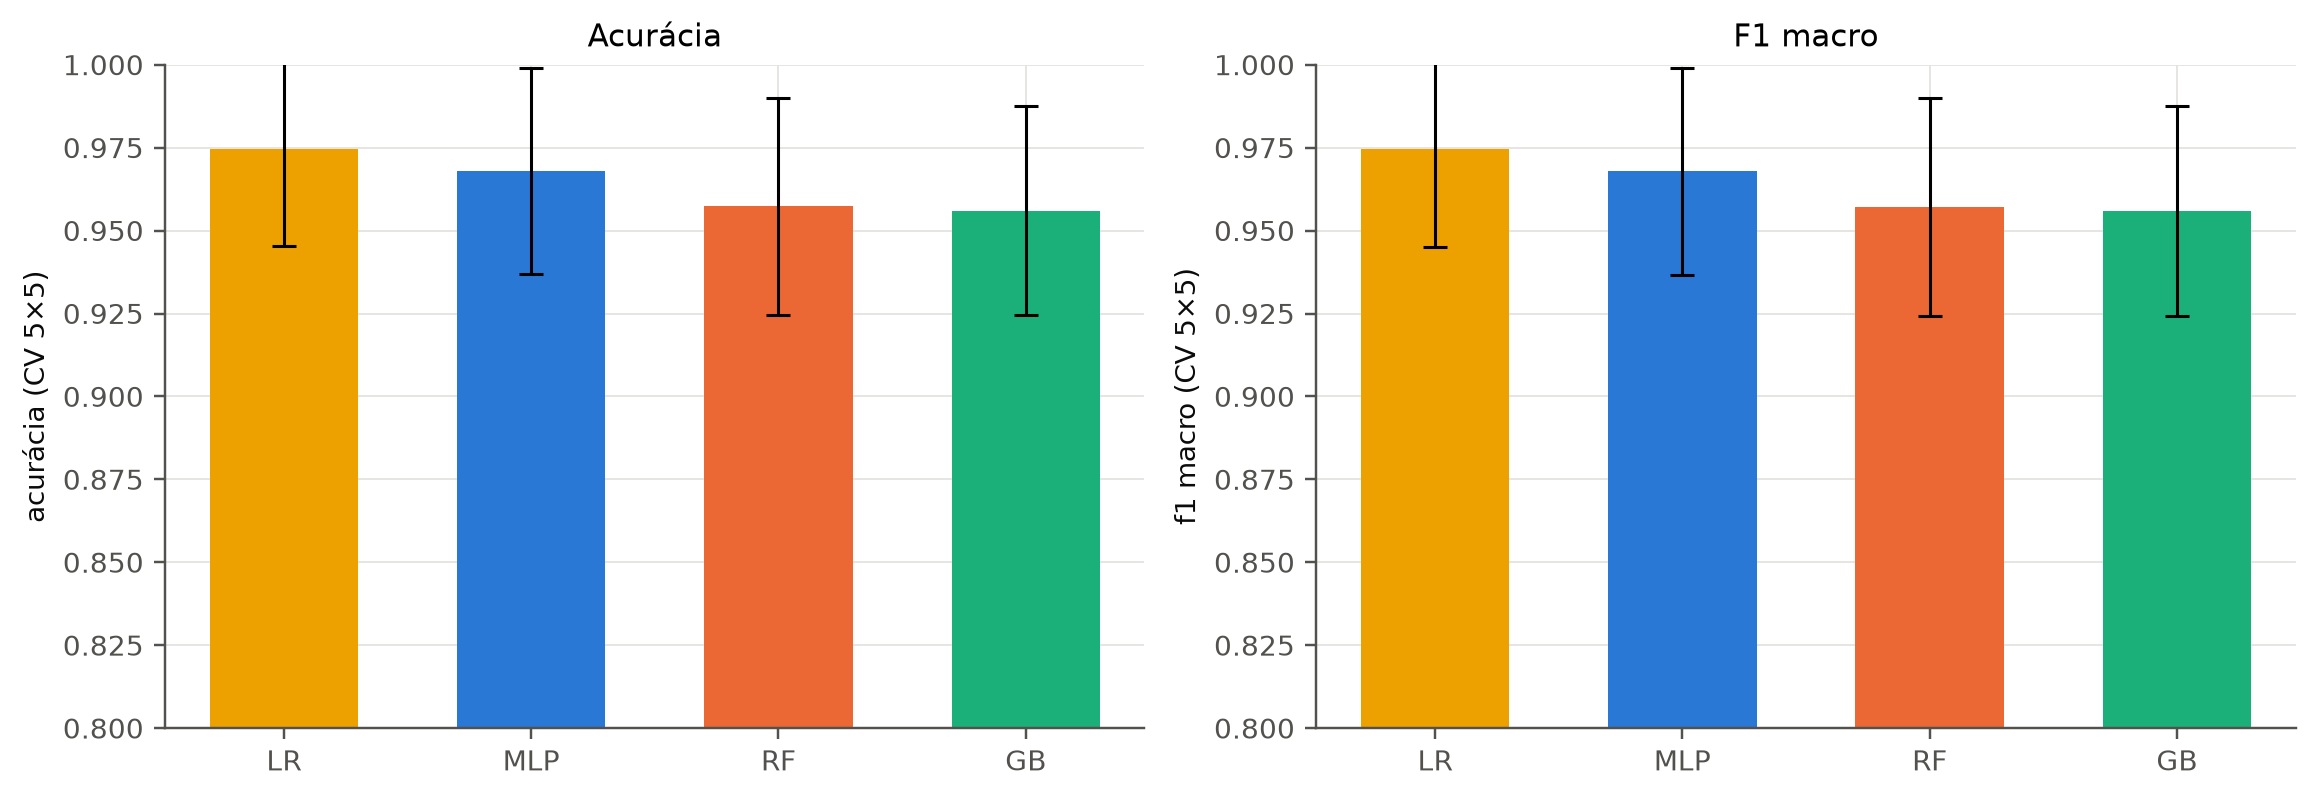
\includegraphics[width=\textwidth]{fig_comparacao_modelos.png}
	\caption{Acurácia e $F_1$ macro dos quatro modelos (validação cruzada 5 $\times$ 5). As barras
	de erro são $\pm 1$ desvio-padrão entre as 25 dobras.}
	\label{fig:comparacao}
\end{figure}

A ordenação é: regressão logística (\accLR{}), MLP (\accMLP{}), floresta aleatória (\accRF) e
\emph{gradient boosting} (\accGB). A regressão logística vence --- e vence com folga de tempo:
seus 25 ajustes levam uma fração de segundo, cerca de quarenta vezes menos que os da MLP
(\tabela{tab:modelos}).

A \tabela{tab:testes} traz o teste de Wilcoxon pareado para as três comparações.

\begin{table}[htbp]
	\centering
	\caption{Teste de Wilcoxon pareado entre a MLP e os demais modelos, sobre as 25 dobras de
	validação cruzada. A diferença é medida em pontos percentuais (MLP menos o outro modelo).}
	\label{tab:testes}
	% gerado automaticamente por mlp_iris.py - nao editar

\begin{tabular}{lrrr}
\toprule
\textbf{comparação} & \textbf{estatística W} & \textbf{valor p} & \textbf{diferença (p.p.)} \\
\midrule
MLP $\times$ RF & 3,5 & 0{,}033 & 1,07 \\
MLP $\times$ GB & 5,0 & 0{,}013 & 1,20 \\
MLP $\times$ LR & 0,0 & 0{,}025 & -0,67 \\
\bottomrule
\end{tabular}

\end{table}

As três diferenças são estatisticamente significativas ao nível de $5\,\%$: a MLP é melhor que a
floresta ($+1{,}07$ p.p., $p=\pRF$) e que o \emph{boosting} ($+1{,}20$ p.p., $p=\pGB$), e pior
que a regressão logística ($-0{,}67$ p.p., $p=\pLR$).

\paragraph{Como interpretar.} A significância estatística aqui mede consistência, não magnitude.
Uma diferença de $0{,}67$ ponto percentual é irrelevante na prática: corresponde a uma amostra em
150. O que os números realmente dizem é que, no Iris, os quatro modelos são essencialmente
equivalentes, e que qualquer afirmação de superioridade precisa de um conjunto maior para se
sustentar. A regressão logística leva vantagem por ser mais simples, mais rápida e igualmente
precisa --- exatamente o tipo de conclusão que o princípio da parcimônia recomenda.

\subsection{Efeito da padronização}

A \figura{fig:escala} compara o treinamento com e sem padronização, para Adam e para SGD com
momento.

\begin{figure}[htbp]
	\centering
	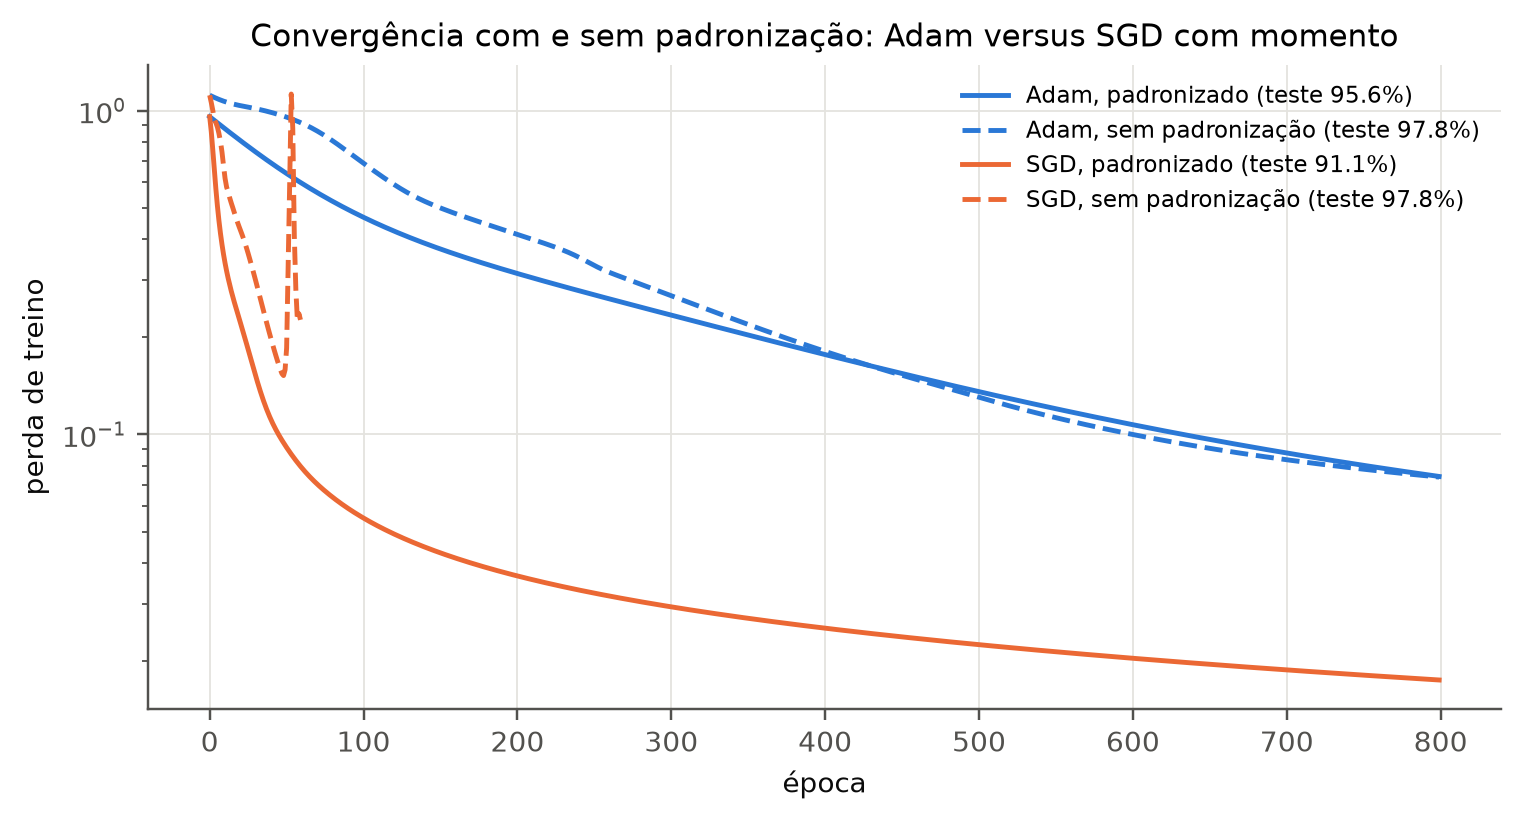
\includegraphics[width=0.82\textwidth]{fig_escala.png}
	\caption{Curvas de perda com e sem padronização dos atributos, para Adam (linhas contínuas) e
	SGD com momento (tracejadas). A acurácia indicada é a do conjunto de teste.}
	\label{fig:escala}
\end{figure}

Os resultados confirmam a teoria. Com Adam, as curvas com e sem padronização são quase idênticas:
o otimizador normaliza o passo por parâmetro e, por isso, é pouco sensível à escala. Com SGD, a
mesma taxa de aprendizado produz trajetórias muito diferentes: a versão sem padronização converge
em 60 épocas para uma perda de $0{,}23$, enquanto a versão padronizada precisa das 800 épocas para
chegar a $0{,}017$. A taxa adequada a uma escala não é adequada à outra.

A lição é prática: a padronização não é um ritual, é uma forma de tornar o problema independente
da escolha de taxa de aprendizado. Quando se usa um otimizador adaptativo como o Adam, ela é
quase cosmética; quando se usa SGD puro, ela é essencial. No Iris, como os atributos já estão em
centímetros e em faixas parecidas, o efeito sobre a acurácia final é pequeno --- mas o experimento
mostra por que o procedimento é adotado por padrão.

\subsection{Resumo dos resultados}

A \tabela{tab:resumo} consolida os números principais.

\begin{table}[htbp]
	\centering
	\caption{Síntese dos resultados do modelo principal.}
	\label{tab:resumo}
	\small
	\begin{tabular}{L{7.4cm} R{3.2cm}}
		\toprule
		\textbf{Item} & \textbf{Valor} \\
		\midrule
		Amostras (treino / teste) & \nTreino{} / \nTeste{} \\
		Atributos / classes & 4 / 3 \\
		Arquitetura & 4--16--3 \\
		Parâmetros treináveis & \parametrosMLP{} \\
		Acurácia (validação cruzada 5 $\times$ 5) & 96,8\,\% \\
		Acurácia (teste, $n=45$) & \accTeste{} \\
		Intervalo de confiança de Wilson (95\,\%) & [\icLo{}; \icHi{}] \\
		$F_1$ macro (teste) & \fmacroTeste{} \\
		Entropia cruzada (teste) & \llteste{} \\
		Épocas até a parada antecipada & \nIter{} \\
		Erro relativo máximo do gradiente & \erroGrad{} \\
		Acurácia da implementação em NumPy & \accNumpy{} \\
		\bottomrule
	\end{tabular}
\end{table}
